%-------------------------------PPT Title-------------------------------------
\title{刘曾复教授对我国生理学科的贡献}
%-----------------------------------------------------------------------------

%----------------------------Author & Date------------------------------------
\author[\textrm{Jun\_Jiang}]{姜~骏\inst{}
%\vskip -20pt 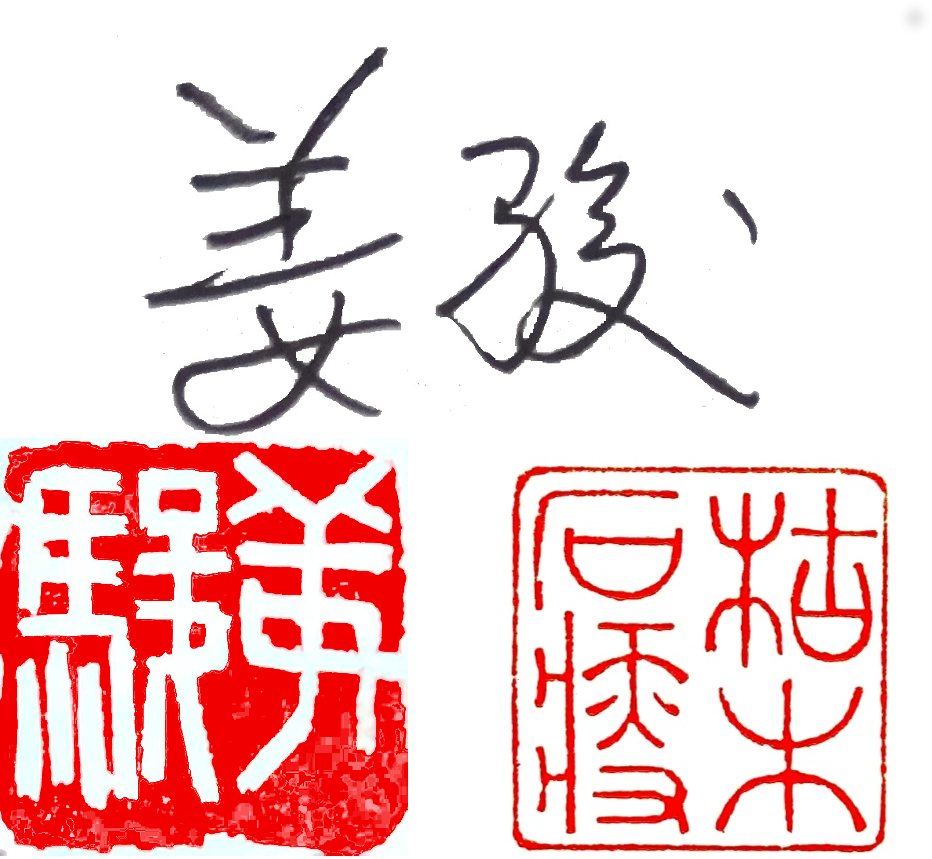
\includegraphics[scale=0.03]{Figures_Peking-Opera/signature-seal_Jiang-1.png} % 加入个人名章 
%\vskip 2pt 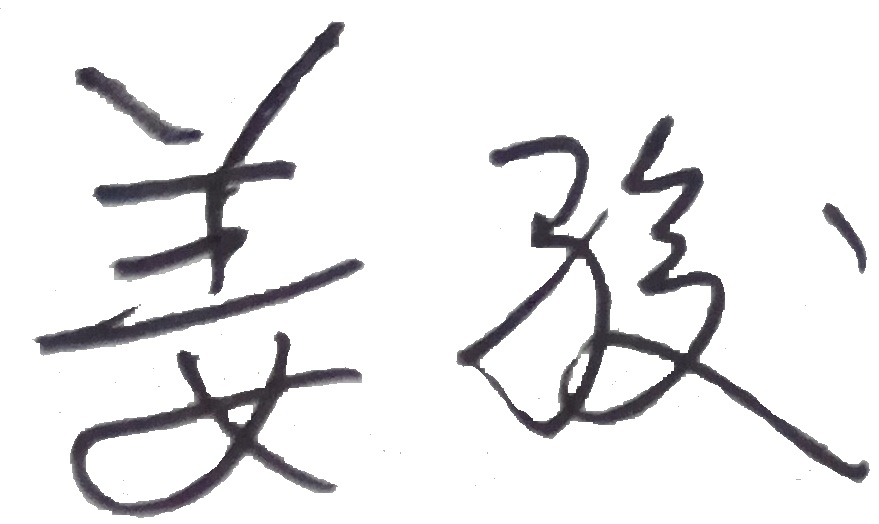
\includegraphics[scale=0.06]{Figures_Peking-Opera/signature_Jiang_new.jpg} % 加入个人签名 
%\vskip -20pt 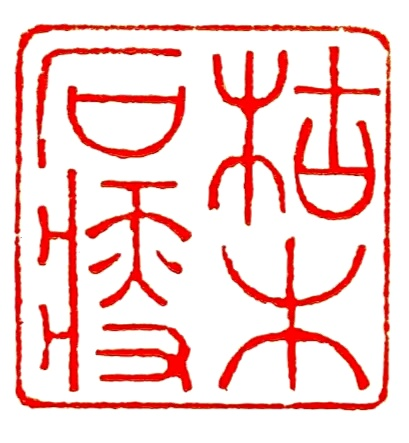
\includegraphics[scale=0.11]{Figures_Peking-Opera/seal_Jiang-2.jpg} % 加入个人闲章 
} %[]{} (optional, use only with lots of authors)
% - Give the names in the same order as the appear in the paper.
% - Use the \inst{?} command only if the authors have different
%   affiliation.
%\institute[BCC]{\inst{}%
 \vskip -30pt %北京市计算中心}
\date[\today] % (optional, should be abbreviation of conference name)
{	{\fontsize{6.2pt}{4.2pt}\selectfont{\textcolor{blue}{E-mail:~}\url{czjiangjun@yeah.cn}}}
\vskip 10 pt {\fontsize{8.2pt}{6.2pt}\selectfont{%报告地点   %清华大学\;\;物理系   
\vskip 5 pt \textrm{2024.12.19}}}
}

% - Either use conference name or its abbreviation
% - Not really information to the audience, more for people (including
%   yourself) who are reading the slides online

% This is only inserted into the PDF information catalog. Can be left
% out.
\frame[allowframebreaks]
{
	\frametitle{\fontsize{9.5pt}{5.2pt}\selectfont{\textcolor{orange}{``居今稽古''纪念刘曾复教授诞辰110周年}}}
\titlepage
}
%-----------------------------------------------------------------------------

\logo{}
%------------------------------------------------------------------------------列出全文 outline ---------------------------------------------------------------------------------
\section*{}
\frame[allowframebreaks]
{
  \frametitle{Outline}
%  \frametitle{\textcolor{mycolor}{\secname}}
  \tableofcontents%[current,currentsection,currentsubsection]
}
%在每个section之前列出全部Outline
%类似的在每个subsection之前列出全部Outline是\AtBeginSubsection[]
\AtBeginSection[]
{
  \frame<handout:0>%[allowframebreaks]%讲义(handout)不显示 <handout:0> 讲义显示 <handout:1> / %beamer不显示 <beamer:0> beamer显示 <beamer:1>	
  {
    \frametitle{Outline}
%全部Outline中,本部分加亮
    \tableofcontents[current,currentsection]
  }
}

%------------------------------------------------------------------------------PPT main Body------------------------------------------------------------------------------------
\small
%\frame
%{
%	\frametitle{引言}
%	2000年左右,随着第一个互联网高峰的到来,戏曲艺术的传播也从传统的广播、电视媒体走向网络。
%}
%\section{求学经历}
\frame
{
	\frametitle{学术简历}
	刘曾复教授(1914-2012)
	\begin{itemize}
		\item 1937年,毕业于清华大学生物学系,获理学学士学位
		\item 1938年12月起,在北平协和医学院生理学系研究实习,开始从事生命科学的研究工作
		\item 1942年因``太平洋战争''爆发,协和医学院教学及医疗工作被迫终止,到中国大学生物系任讲师,直至抗战胜利
		\item 1945年6月至1960年6月期间,在北京医学院(现~北京大学医学部)生理学教研室先后任讲师、副教授、教授,并曾担任基础部副主任
		\item 1960年,奉命由北京医学院调到北京第二医学院(现~首都医科大学),着手组建生理教研室并任主任
		\item 1987年,又受学校委托,组建生物医学工程学系并担任系主任,后担任生物医学工程学院名誉主任
	\end{itemize}
%\begin{figure}[h!] 
%\centering
%\vspace{-0.1in}
%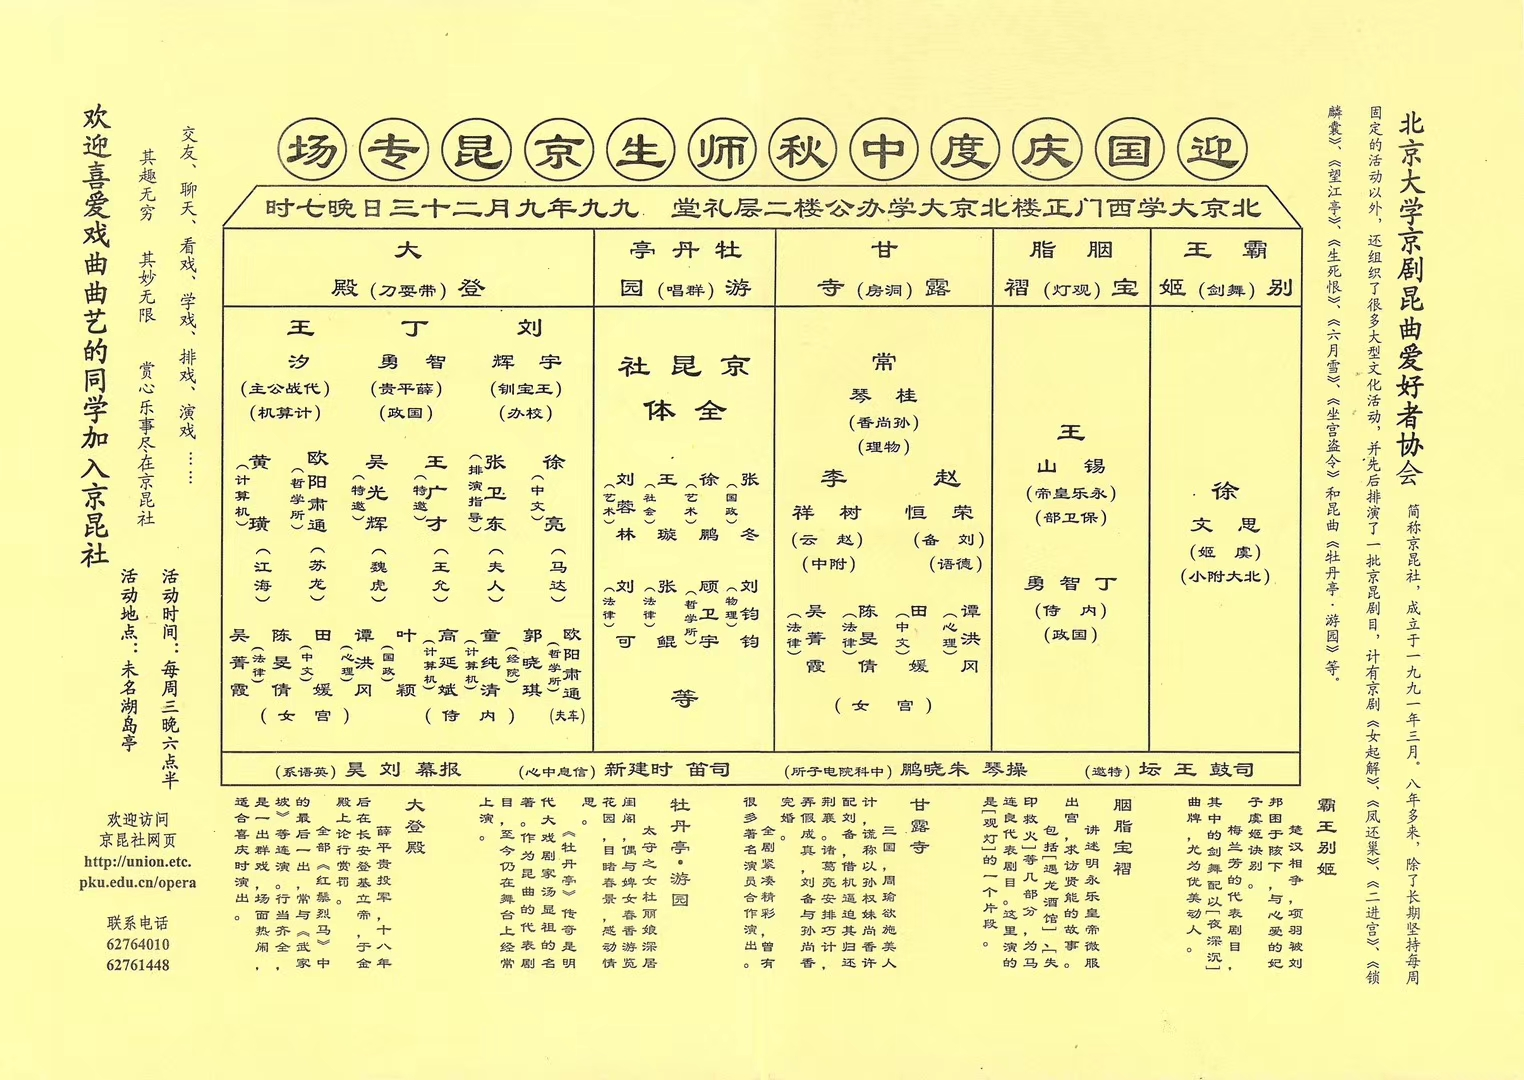
\includegraphics[height=0.70\textwidth,width=0.95\textwidth,clip]{Figures_Peking-Opera/PekOpe_PKU-1.jpg}
%\label{PKU-1}
%\end{figure}
}

\frame{
	\frametitle{对我国生理科学的奠基作用:~讲义与教材}
	早在1940年代,刘曾复教授即已参与相关医学教材的编写
\begin{figure}[h!] 
\centering
\vspace{-0.05in}
\includegraphics[height=0.55\textwidth,width=0.45\textwidth,clip]{Figures_Peking-Opera/Liu-Physiology-Pratice_2.jpg}
\includegraphics[height=0.55\textwidth,width=0.45\textwidth,clip]{Figures_Peking-Opera/Liu-Physiology-Pratice_3.jpg}
\label{Liu-Anatomy_and_Physiology-practice}
\end{figure}
}

\frame
{
	\frametitle{对我国生理科学的奠基作用:~讲义与教材}
	在1950-1960年代,刘曾复教授主持编写的生理学教材,在全国中等、高等医学院校广泛使用,重印多次
\begin{figure}[h!] 
\centering
\vspace{-0.05in}
\includegraphics[height=0.45\textwidth,width=0.33\textwidth,clip]{Figures_Peking-Opera/Liu-Anatomy_and_Physiology-1.jpg}
\includegraphics[height=0.45\textwidth,width=0.33\textwidth,clip]{Figures_Peking-Opera/Liu-Anatomy_and_Physiology-3.jpg}
\includegraphics[height=0.18\textwidth,width=0.40\textwidth,viewport=0 70 1071 630,clip]{Figures_Peking-Opera/Liu-Anatomy_and_Physiology-2.jpg}
\label{Liu-Anatomy_and_Physiology-middle}
\end{figure}
}

\frame
{
	\frametitle{对我国生理科学的奠基作用:~讲义与教材}
\begin{figure}[h!] 
\centering
\vspace{-0.05in}
\includegraphics[height=0.48\textwidth,width=0.35\textwidth,clip]{Figures_Peking-Opera/Liu-Anatomy_and_Physiology-5.jpg}
\includegraphics[height=0.48\textwidth,width=0.35\textwidth,clip]{Figures_Peking-Opera/Liu-Anatomy_and_Physiology-7.jpg}
\includegraphics[height=0.22\textwidth,width=0.45\textwidth,viewport=0 70 548 330,clip]{Figures_Peking-Opera/Liu-Anatomy_and_Physiology-6.jpg}
\label{Liu-Anatomy_and_Physiology-college}
\end{figure}
}

\frame
{
	\frametitle{生理科学研究的贡献:~代表论文与专著}
	刘曾复教授毕生的研究经历
	\begin{itemize}
		\item 普通生理学:~垂体活动、代谢与消化的神经与体液调节

		\item 电生理学\\
陈兰生、刘曾复、沈寯淇, 蟾蜍中枢神经系统的抑制过程和脑电图的关系,生理学报, 24(1), 47, 1960\\
王雨若、张英才、赵紫东、刘曾复,刺激迷走神经对皮层诱发性下颌运动的抑制作用,生理学报,26(3), 251, 1963
		\item 神经系统的整合作用研究\\
刘曾复、丁延衸、赵以炳, 控制理论与生理控制系统,生理科学进展,9(2),97, 1978
	\end{itemize}
}

\frame
{
	\frametitle{对我国生理科学的奠基作用:~论文与专著}
	进入1980年代,随着科研活动的重新进展,刘曾复教授出版专著并极为重视数学在生理科学中的应用
\begin{figure}[h!] 
\centering
\vspace{-0.05in}
\includegraphics[height=0.55\textwidth,width=0.40\textwidth,clip]{Figures_Peking-Opera/Liu-Neurophysiology-1.jpg}
%\includegraphics[height=0.48\textwidth,width=0.35\textwidth,clip]{Figures_Peking-Opera/Liu-Neurophysiology-2.jpg}
\includegraphics[height=0.55\textwidth,width=0.40\textwidth,clip]{Figures_Peking-Opera/Liu-Mathematic.jpg}
\label{Liu-Anatomy_and_Physiology-college}
\end{figure}
}

\frame
{
	\frametitle{刘曾复先生:~科学整合的思想}
	尝试用现代科学的文字和符号,建立关于京剧表演中基本核心技术传承的语言体系
。
\begin{figure}[h!]
\centering
\vspace{-0.2in}
%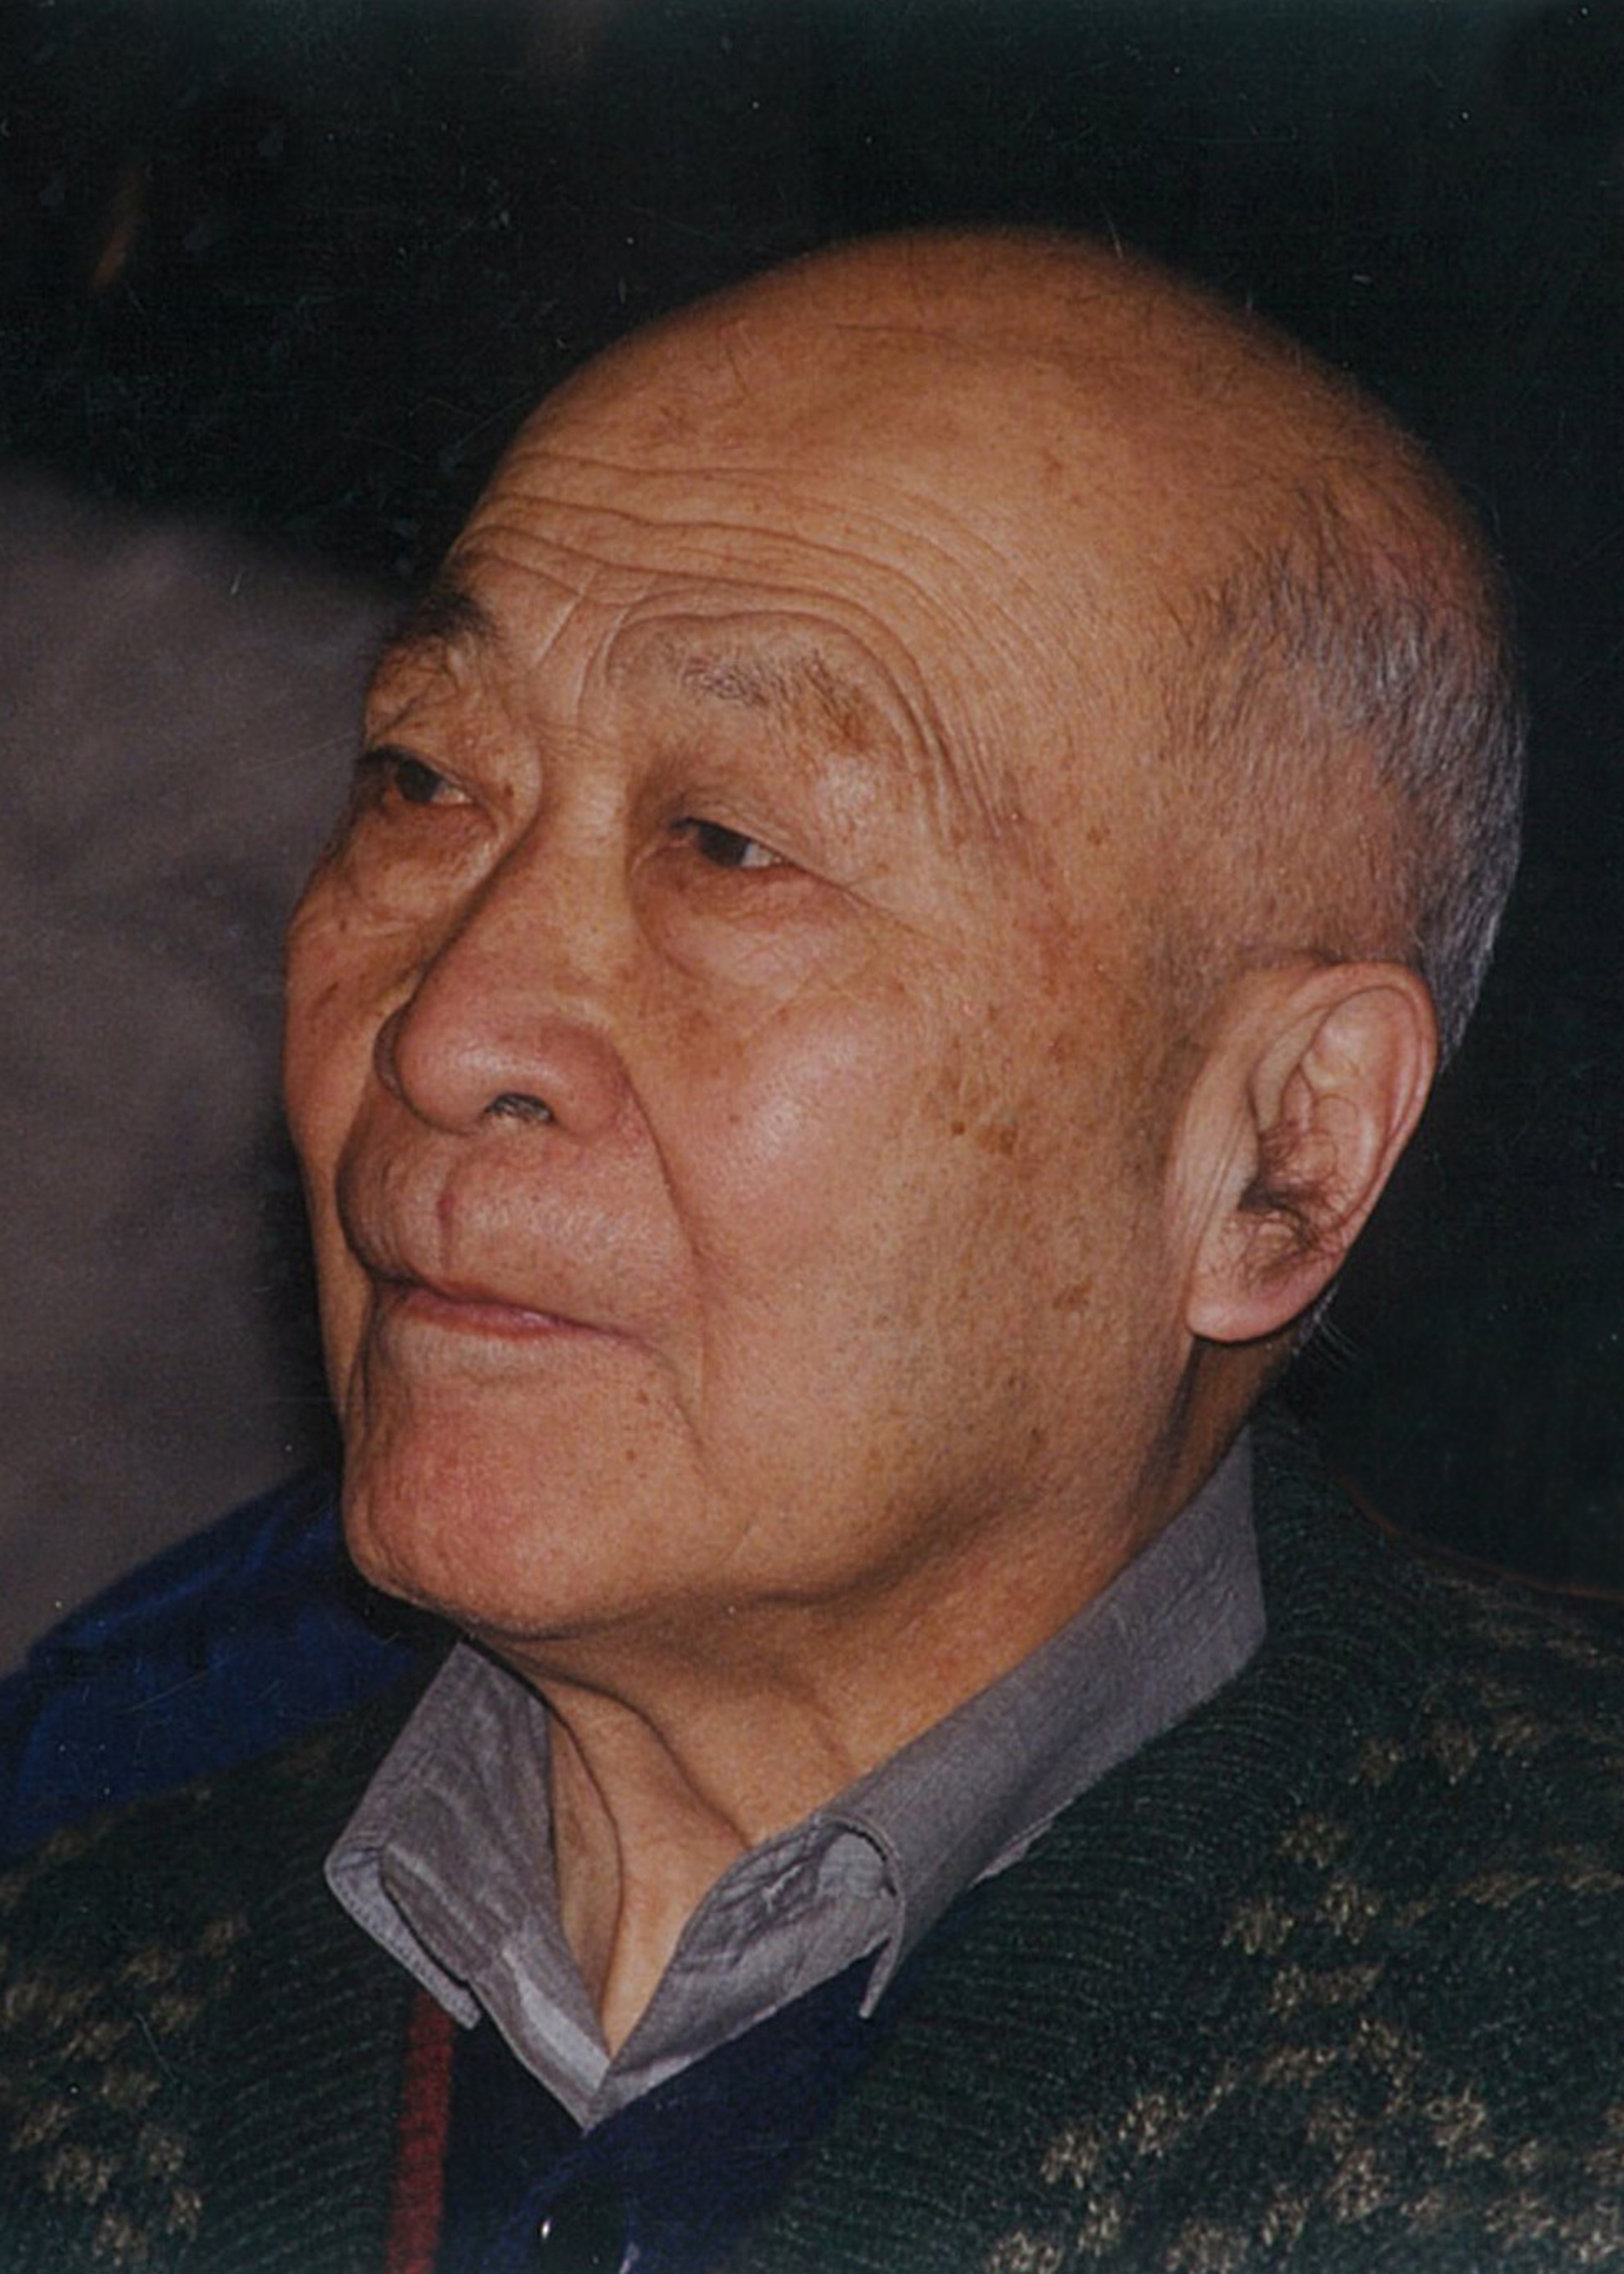
\includegraphics[height=0.64\textwidth,width=0.46\textwidth,viewport=0 0 360 520,clip]{Figures_Peking-Opera/Liu_Zengfu.jpg}
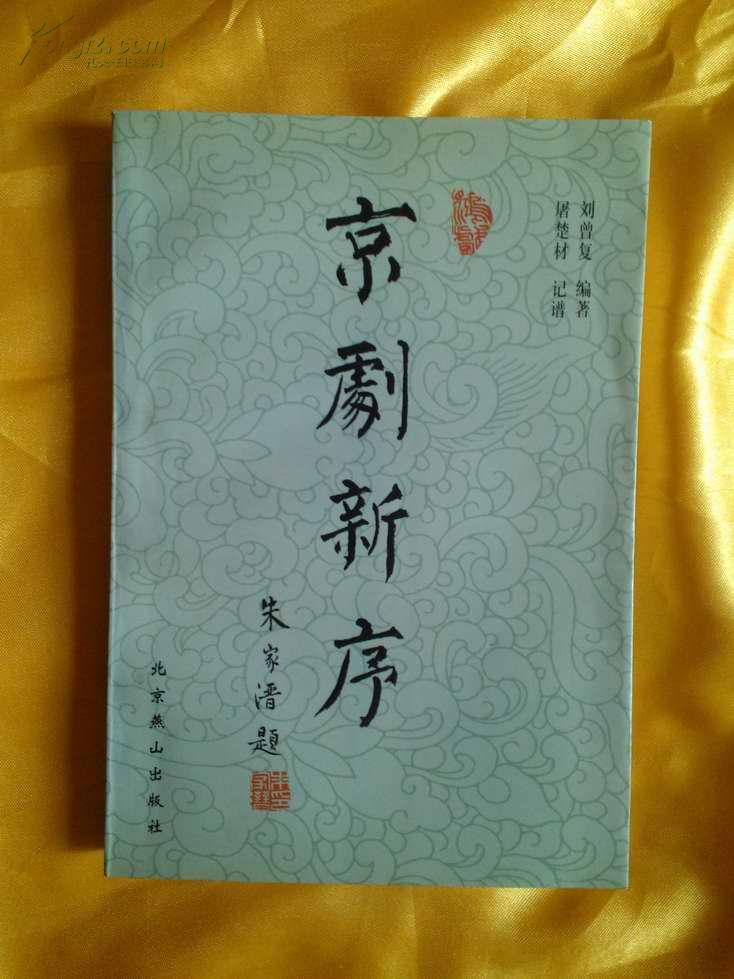
\includegraphics[height=0.62\textwidth,width=0.45\textwidth,viewport=100 85 660 875,clip]{Figures_Peking-Opera/Liu_Xinxu.jpg}
\hskip 5pt
\includegraphics[height=0.62\textwidth,width=0.45\textwidth,viewport=0 0 230 185,clip]{Figures_Peking-Opera/Broad_spectrum-analysis.jpg}
%\caption{刘曾复先生}
\label{Liu_Xinxu}
\end{figure}
}

%\frame
%{
%	\frametitle{答辩合影}
%\begin{figure}[h!]
%\centering
%\vspace{-10.5pt}
%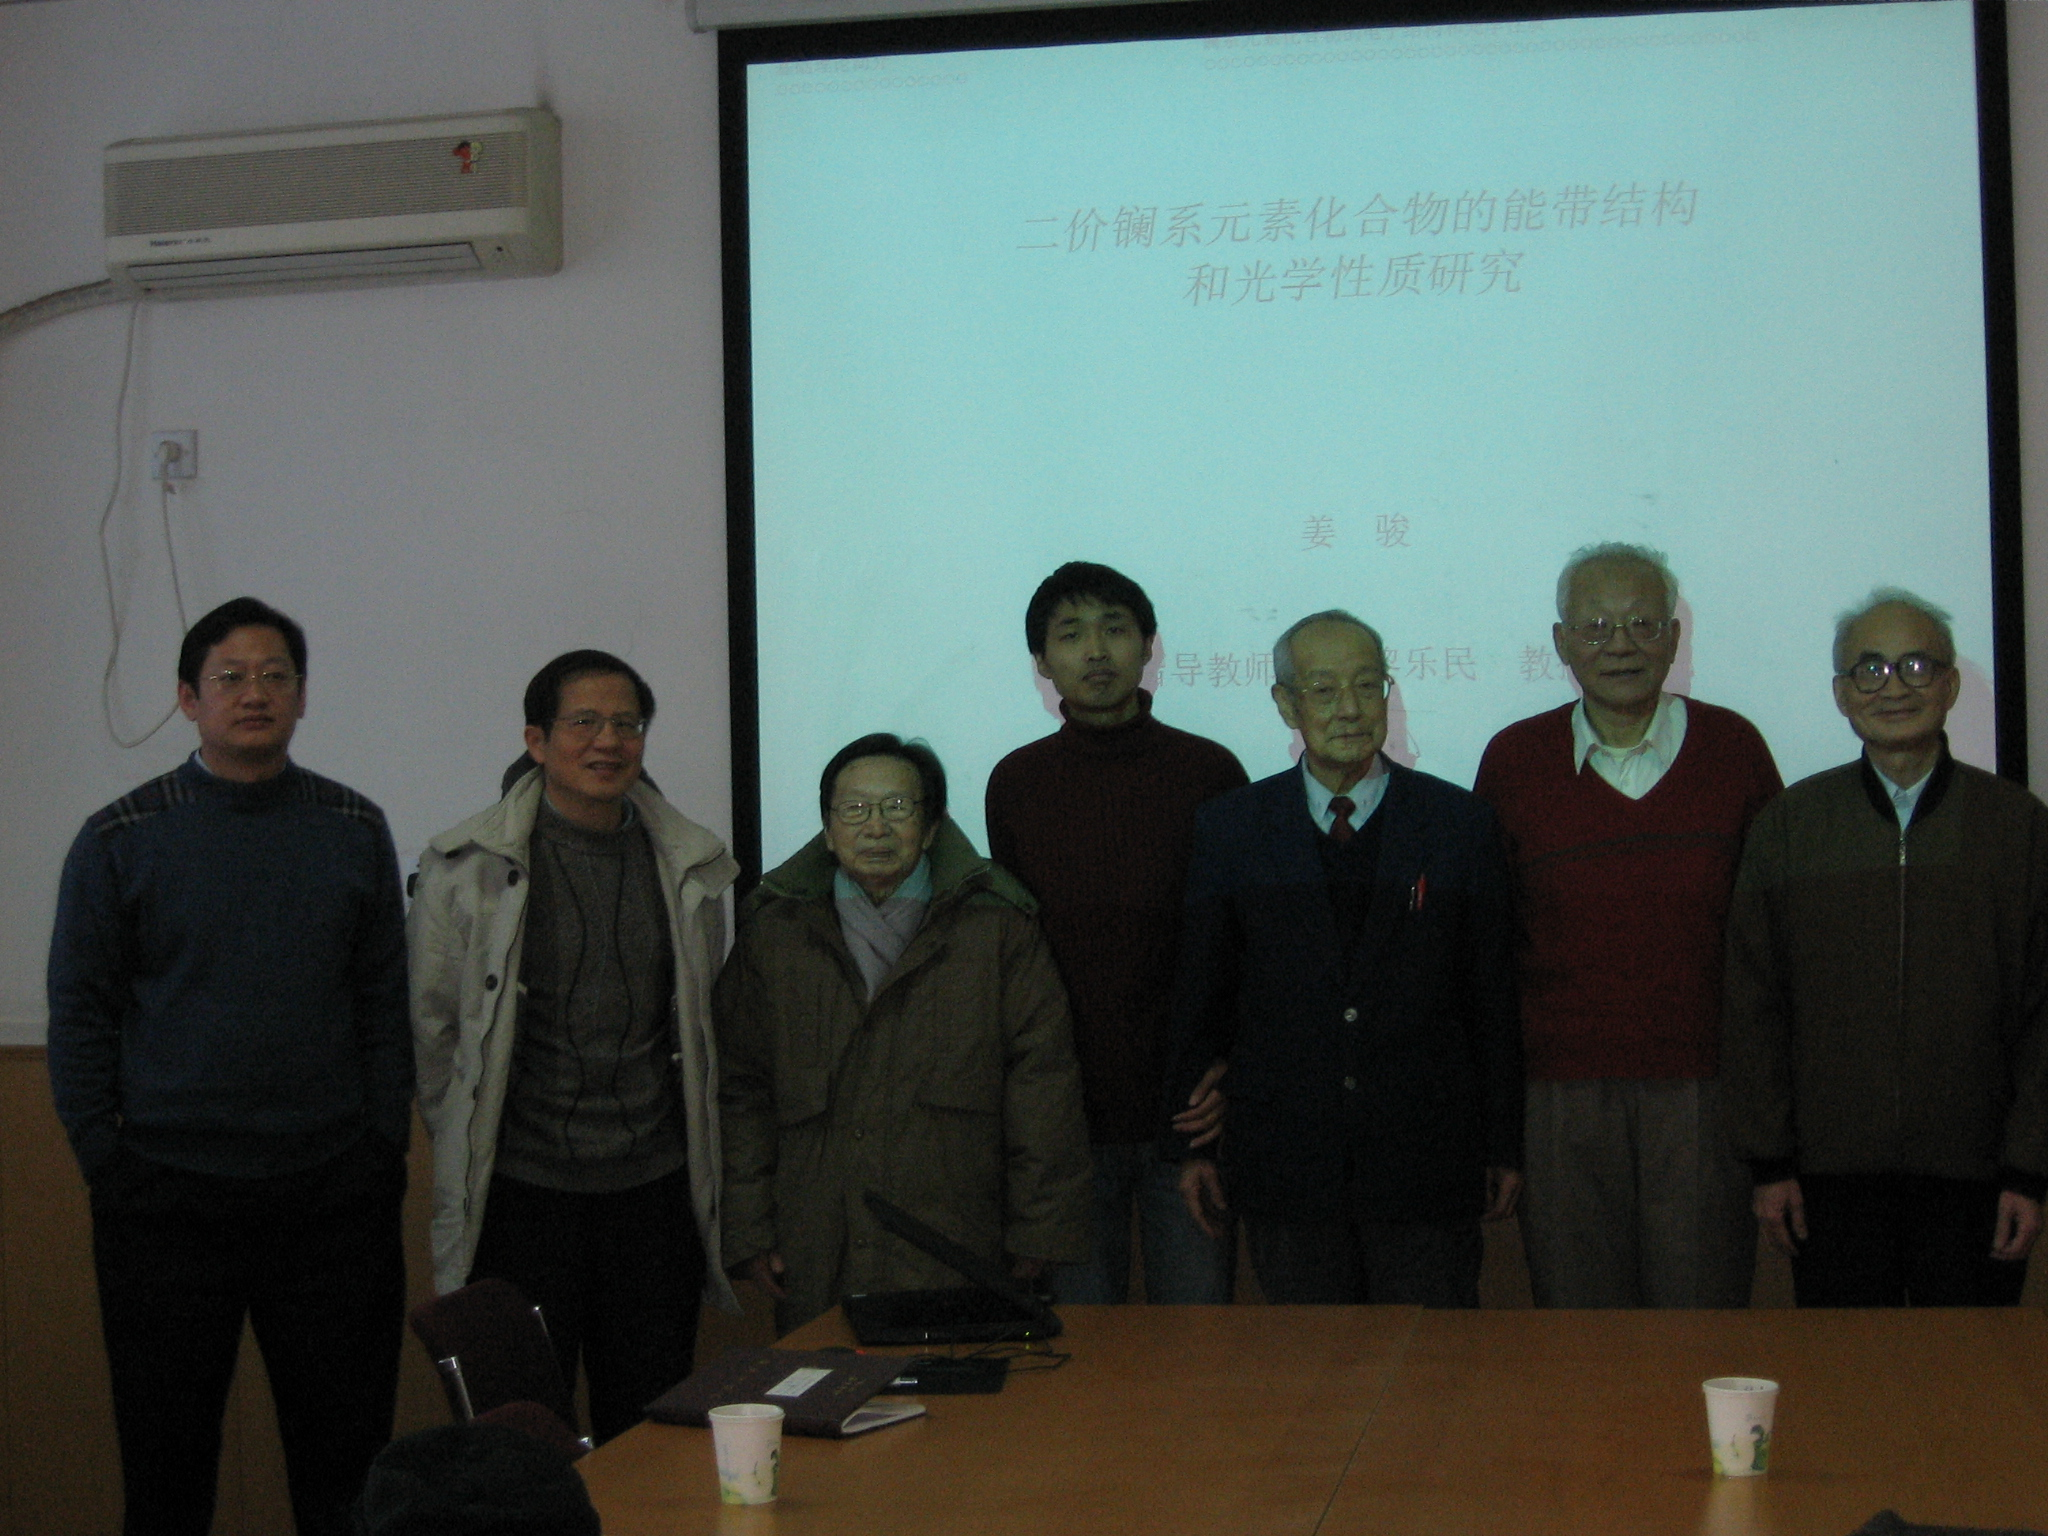
\includegraphics[height=0.62\textwidth,width=0.9\textwidth,viewport=0 0 820 600,clip]{Figures_Peking-Opera/Thesis_Defense_2007.jpg}
%\caption{\textrm{2007.12.15博士论文答辩后留影:}\\{\fontsize{7.1pt}{3.9pt}\selectfont\textrm{左起:~刘文剑教授、黄元河教授、刘若庄教授、答辩人、徐光宪教授、王德民教授、黎乐民教授}}}
%\label{Thesis_Defense_2007}
%\end{figure}
%}

%\frame
%{
%	\frametitle{说戏剧本集}
%\begin{figure}[h!]
%\centering
%\vspace{-10.5pt}
%\includegraphics[height=0.68\textwidth,width=0.49\textwidth,viewport=0 0 1030 1400,clip]{Figures_Peking-Opera/Liu_script.jpg}
%\includegraphics[height=0.68\textwidth,width=0.125\textwidth,viewport=0 0 620 2850,clip]{Figures_Peking-Opera/Liu_script-Inscription.JPG}
%\caption{\fontsize{6.1pt}{3.9pt}\selectfont\textrm{《刘曾复说戏剧本集》~陈佩秋题签~~华东师范大学出版社~(2015.08)}}
%\label{Peking_Opera_Script-2015}
%\end{figure}
%}

%\frame
%{
%	\frametitle{京剧唱腔选}
%\begin{figure}[h!]
%\centering
%\vspace{-10.5pt}
%\includegraphics[height=0.65\textwidth,width=0.95\textwidth,viewport=0 0 680 450,clip]{Figures_Peking-Opera/Wu_CD.jpg}
%\caption{\fontsize{6.1pt}{3.9pt}\selectfont\textrm{《吴小如京剧唱腔选》~绝版赏析栏目组~~新汇集团上海音像有限公司~(2013.03)}}
%\label{Peking_Opera_CD-2012}
%\end{figure}
%}

\section{自媒:~分化与新生代}
\frame
{
	\frametitle{自媒体时代的到来}
	\begin{itemize}
                \setlength{\itemsep}{20pt}
		\item \textrm{2010}年左右,随着微博、微信的出现,戏曲业余爱好者交流的方式日趋多元,戏曲资源和资料以短的多媒体形式传播越发便捷
		\item \textrm{2016}年左右,随着网易云音乐、喜马拉雅、抖音、\textrm{Bilibili}等自媒体的发达,特别是\textrm{1995/2000}后的小朋友们成为网络的主力,一批新的传统戏曲爱好者正在引领潮流
		\item \textrm{1970/80}后的戏迷也有不少加入了自媒体戏曲推广的行列,但总体来说,他们的方式更传统一些,在\textrm{1995/2000}后的眼中,一如他们自己年轻时眼中的父辈
	\end{itemize}
}

\frame
{
	\frametitle{网络交流的价值:~以余叔岩为例}
网络大大方便了获取学习、了解余派资料的途径
\begin{itemize}
	\item 数字化的说戏录音:~陈少霖、孟小冬及其弟子、再传
	\item 李适可传于世文的说戏录音、录像
	\item 余派研究资料:\\
		《谈余叔岩》、《余叔岩与余派艺术》、《余叔岩年谱》
\end{itemize}
\vskip 3pt
个人的思考:~面对旦行的崛起,余叔岩作出可贵的探索
\begin{itemize}
%   \setlength{\itemsep}{20pt}
	\item 对谭派的继承:~体现在所演出剧目的\textcolor{blue}{全面性}
	\item 对谭派的发展:~体现在所演出剧目的\textcolor{blue}{选择性}
	\item \textcolor{blue}{表演的格调和气质}:~知取舍
\end{itemize}
%业余爱好者和内行专业人士参考:
\vskip 5pt
%但也是一条险峻而艰难的道路
\textcolor{red}{余叔岩的创新:~绝不体现在新编剧目上}
}


%\begin{frame}
%	\frametitle{frame with sound}
%\dots
%\includemedia[ 
%	label=my_sound,
%	width=1ex, height=1ex, 
%	transparent,
%	activate=pageopen, 
%	deactivate=onclick,
%	addresource=Figures_Peking-Opera/Liu-Xiongzhouguan.mp3,
%	flashvars={source=Figures_Peking-Opera/Liu-Xiongzhouguan.mp3
%                  &autoPlay=true
%                  &loop=true
%                  &hideBar=false}
%	  ]{}{APlayer.swf}
%\dots
%\end{frame}

%\begin{frame}{other frame}
%\dots
%\end{frame}

%\pdfpageattr{/AA <</O <</S/JavaScript/JS (annotRM['my_sound'].activated=false;)>> >>}
%\begin{frame}{frame where sound stops}
%\dots
%\end{frame}

%\begin{frame}{another dumb frame}
%\dots
%\end{frame}

%%%%%%%%%%%%%%%%%%%%%%%%%%%%%%%%%%%%%%%%%%%%%%%%%%%%%%%%%%%%%%%%%%%%%%%%%%%%%%%%%%%%%%%%%%%%%%%%%%%%%%%%%%%%%%%

%\frame<handout:0>
%{
%	\frametitle{}
%\begin{figure}[h!]
%\centering
%\animategraphics[autoplay, loop, height=2.0in]{1}{Figures_Peking-Opera/vlcsnap-}{01}{10}
%\label{Pro_Liu_gif}
%\end{figure}
%}

%%%%%%%%%%%%%%%%%%%%%%%%%%%%%%%%%%%%%%%%%%%%%%%%%%%%%%%%%%%%%%%%%%%%%%%%%%%%%%%%%%%%%%%%%%%%%%%%%%%%%%%%%%%%%%%

%------------------------------------------------------------------------Reference----------------------------------------------------------------------------------------------
%\begin{thebibliography}{99}
%-----------------------------------------------------------------------------------------------------------------------------------------------------------------------%
%\frame
%{
%\frametitle{主要参考文献}
%{\small
%\bibitem{Singh_Book}\textrm{D. J. Singh. \textit{Plane Wave, PseudoPotential and the LAPW method} (Kluwer Academic, Boston,USA, 1994)}					%
%  \nocite{*}																				%
%}
%}
%\end{thebibliography}
%\frame%[allowframebreaks]
%{
%\begin{thebibliography}{99}
%\frametitle{主要参考文献}
%{\small
%	\bibitem{Zhu_Tuishilu}朱家溍 著, {\textit{故宫退食录}}\;\textrm{({\textit{上、下}})}\:北京出版社, 北京, 1999\\
%朱家溍 著, {\textit{故宫退食录}}\;\textrm{({\textit{上、下}})}\:紫禁城出版社, 北京, 2009
%	\bibitem{Liu_Xinxu}刘曾复 编著、屠楚材 记谱, {\textit{京剧新序}}\:燕山出版社, 北京, 1999\\
%{\fontsize{7.0pt}{3.9pt}\selectfont 刘曾复 编著、屠楚材 记谱,娄悦、何毅 整理, {\textit{京剧新序}}\;\textrm{(修订版)}\:学苑出版社, 北京, 2009}\\
%刘曾复 传述, {\textit{刘曾复说戏剧本集}}\:华东师范大学出版社, 上海, 2015
%	\bibitem{Wu_Wenlu}吴小如 著, {\textit{吴小如戏曲文录}}\:北京大学出版社, 北京, 1995 \\
%	吴小如 著, {\textit{吴小如戏曲随笔集补编}}\:天津古籍出版社, 天津, 2006
%	\bibitem{XQYS1-32_1983}\textrm{刘曾复、王世续、王金彦, 京剧老生把子见闻录\:\textit{戏曲艺术}, \textbf{第一期} (1983), 32}
%	\bibitem{ZGXJ1-57_1993}\textrm{刘曾复, 京剧书文指伪录\:\textit{中国戏剧}, \textbf{第01期} (1993), 57}
%}
%\nocite*{}
%\end{thebibliography} 
%}

%-----------------------------------------------------------Beamer下不建议使用bib,因为涉及分页--------------------------------------------------------------------------%
\frame[allowframebreaks]
{
\frametitle{主要参考文献}
{\tiny\textrm{
%%\phantomsection\addcontentsline{toc}{section}{Bibliography}	 %直接调用\addcontentsline命令可能导致超链指向不准确,一般需要在之前调用一次\phantomsection命令加以修正	%
%%\phantomsection\addcontentsline{toc}{section}{主要参考文献}	 %直接调用\addcontentsline命令可能导致超链指向不准确,一般需要在之前调用一次\phantomsection命令加以修正	%
\bibliography{Peking_Opera}%
%\bibliographystyle{../ref/mybib}%
\bibliographystyle{plain}%
\vskip 8pt
部分资料参阅了戏考\textrm{blog}({\url{https://blog.xikao.com/}})的纪录\\其余资源引自网络,恕未一一注明出处}}
\nocite{*}
}
%{\small
%\phantomsection\addcontentsline{toc}{section}{Bibliography}	 %直接调用\addcontentsline命令可能导致超链指向不准确,一般需要在之前调用一次\phantomsection命令加以修正	%
%\bibliography{Myref}																			%
%\bibliographystyle{mybib}																		%
%  \nocite{*}																				%
%}

%------------------------------------------------------------------------------------------------------------------------------------------------------------------------------%

%%%%%%%%%%%%%%%%%%%%%%%%%%%%%%%%%  插入音频/视频,使用url 要求视频在指定目录下 %%%%%%%%%%%%%%%%%%%%%%%%%%%%%%%%
%%%%%%%%%%%%%%%%%%%%%%%%%%%%%%%%%%%%%%%%%%%%%%%%%%%%%%%%%%%%%%%%%%%%%%%%%%%%%%%%%%%%%%%%%%%%%%%%%%%%%%%%%%%%%%%
\frame<handout:0>										 	      %
{													      %
	\frametitle{京剧名宿遗音}									      %
\begin{figure}[ht]											      %
%	\includemovie[poster, autostart,controls, mouse, url, text=(xx), repeat] {0.8\textwidth}{0.6\textwidth}{traffic.avi}		      %
%	\includemovie[poster, controls, mouse, url] {0.8\textwidth}{0.6\textwidth}{traffic.avi}		      %
	%\includemovie[poster, controls, mouse, url] {0.8\textwidth}{0.6\textwidth}{Yuan_Kuocheng.mp4}	      %
	\includemovie[poster, controls, mouse, url] {0.8\textwidth}{0.2\textwidth}{Figures_Peking-Opera/Liu-Xiongzhouguan.mp3}     %
	\includemovie[poster, controls, mouse, url] {0.8\textwidth}{0.2\textwidth}{Figures_Peking-Opera/Zhu_Liu-Luomahu.mp3}	      %
%	\includemovie[poster, controls, mouse, url] {0.8\textwidth}{0.2\textwidth}{Figures_Peking-Opera/Liu-Pantaohui.mp3}	      %
	\includemovie[poster, autostart, mouse, url, repeat] {0.8\textwidth}{0.2\textwidth}{Figures_Peking-Opera/Wu-Pantaohui.mp3}	      %
\caption{京剧名宿遗留音}											      %
\end{figure}												      %
}
